\chapter{Asservissement visuel} \label{chap1}

La vision représente pour les humains environ 70\% des données issues des 
perceptions sensorielles externes \cite{purves2004neuroscience} : d'une 
richesse incroyable, c'est aussi, par conséquent, une source d'erreurs 
inépuisable. La vision artificielle ne déroge pas à ses deux principes, d'où 
l'importance du traitement du signal d'une part (dans le but de recueillir et 
interpréter dans cette grande variété d'informations ce qui est pertinent pour 
une tâche prescrite) et d'une stratégie d'asservissement d'autre part (afin de 
stabiliser une tâche malgré les erreurs et incertitudes sur les données).

Nous allons donc dans un premier temps présenter le mode d'acquisition des 
images, puis nous continuerons sur les modèles de perception utilisés. Une fois 
que nous aurons détaillé la manière dont une scène est projetée sur une image, 
nous pourrons dans une seconde section distinguer plusieurs configurations et 
exposer différentes stratégies d'asservissement pouvant être utilisées. Une 
troisi\`eme section sera consacr\'ee \`a la construction des lois de 
commandes, dont nous fournirons quelques exemples. La quatri\`eme section de ce 
chapitre pr\`esentera les sp\'ecificit\'es d'une utilisation de 
l'asservissement visuel dans le contexte des maipulateurs parall\`eles \`a 
c\^ables : apr\`es avoir pr\'esent\'e les principaux travaux ayant \'et\'e 
effectu\'es dans ce domaine, nous pourrons indiquer les angles d'\'etudes que 
nous avons privil\'egi\'es, les probl\'ematiques aui en \'emergent, et les 
pistes de r\'esolution que nous avons emprunt\'ees.
 
\section{Modèles de capteurs et projections} \label{chap1-0}
 
\subsection{De l'oeil à la caméra} \label{chap1-0-0}
 
Sans pour autant chercher à imiter la vision humaine, la vision artificielle 
s'en inspire néanmoins fortement pour ce qui concerne l'acquisition d'une 
image. Ainsi, pour une caméra, le diaphragme joue le rôle de l'iris et de la 
pupille et détermine la quantité de lumière qui pourra être enregistrée sur un 
intervalle de temps donné. Par la suite, la lentille joue un rôle équivalent à 
la cornée et au cristallin, en faisant converger les rayons lumineux vers la 
rétine sur laquelle sont disséminés environ 125 millions de photorécepteurs : 
c'est au niveau de ces derniers que l'acquisition est véritablement effectuée. 
On distingue parmi les photorécepteurs :
 \begin{figure}[htp]
  \centering
  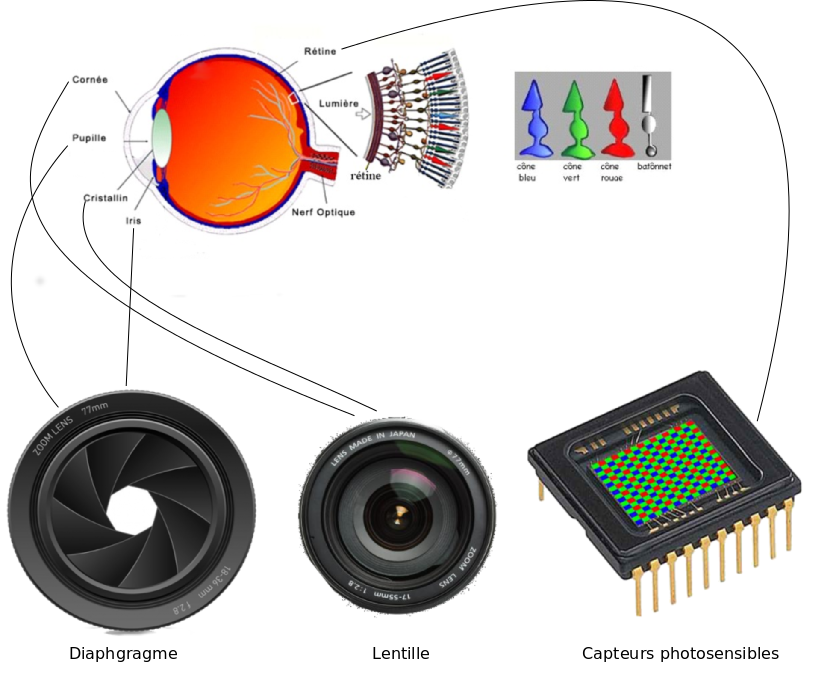
\includegraphics[width=.85\linewidth]{./chapter01/figures/oeil.png}
    \caption{\footnotesize{Oeil humain vs vision artificielle}}
\label{chap01:fig01}
\end{figure}

 \begin{itemize}
  \item les cônes, généralement impliqués dans la vision diurne. Les cônes 
présen\-tent 3 types de pigments leur permettant de réagir à des longueurs 
d'ondes spécifiques (qui ne recouvrent pas exactement le triplet RGB 
traditionnellement utilisé en traitement d'image)
  \item les bâtonnets, impliqués dans la vision nocturne. Ne possédant qu'un 
seul type de pigments, ils ne peuvent pas discriminer les longueurs d'ondes. En 
revanche, ils sont en moyenne 1000 fois plus sensibles à la lumière que les 
cônes, et leur population correspond à 20 fois celle des cônes.
 \end{itemize}

Afin de simuler l'activité des photorécepteurs de l'oeil humain, les 
dispositifs technologiques les plus récents adoptent des stratégies basées sur 
l'utilisation de filtres placés en amont des capteurs photosensibles, 
permettant 
ainsi une acquisition en séquence (un même récepteur recevra successivement les 
réponses des filtres correspondants aux longueurs d'ondes distinguées) ou 
simultanée (les réponses sont envoyées sur des capteurs photosensibles dédiés).
  
L'information contenue dans les données ainsi recueillies est riche et multiple 
: elle peut-être de nature colorimétrique, géométrique, elle permet de 
ca\-ractériser des déplacements, des déformations. Toutefois, ce qui est vu 
n'est jamais qu'une représentation de ce qui est observé : il est d\`es lors 
fondamental d'exploiter les donn\'ees recueillies de mani\`ere \`a tendre 
vers une repr\'esentation exploitable de la scène initiale projetée sur les 
capteurs.

Une premi\`ere option serait de tenter de reconstruire la sc\`ene le plus 
fid\`element possible. On pourra dans ce cas privil\'egier l'utilisation de 
cam\'eras st\'er\'eos (Fig.\ref{chap01:fig02view0})\cite{brandou2006}, ou 
encore de capteurs RGB-D (Fig.\ref{chap01:fig02view1})\cite{siradjuddin2012}. A 
l'aide de cam'eras st\'er\'eos, nous pouvons percevoir la sc\`ene selon 
plusieurs perspectives, tout comme avec la vision binoculaire. En croisant les 
donn\'ees obtenues \`a partir des diff\'erents points de vue, il est possible 
d'approcher une repr\'esentation tri-dimensionnelle de la sc\`ene acquise au 
sein de l'image. Quant aux capteurs RGB-D, ils compl\`etent les donn\'ees 
acquises gr\^ace \`a une ou plusieurs cam\'eras avec de dispositifs permettant 
de recueillir une information sur la profondeur. La fusion des donn\'ees 
g\'eom\'etriques et colorim\'etriques obtenues par les cam\'eras classiques et 
de la localisation tridimensionnelle de points permet une reconstruction 3D de 
la sc\'ene observable. En multipliant les points de vue (soit par le mouvement, 
soit en utilisant plusieurs dispositifs), ou en exploitant un mod\`ele connu de 
la sc\`ene observ\'e, on sera en mesure d'obtenir une repr\'esentation fid\`ele 
d'un environnement. Ce sont toutefois des dispositifs on\'ereux, qui peuvent 
sembler inutilement intrusifs selon le contexte d'utilisation, et requ\'erant 
bien souvent une puissance de calcul d\'emesur\'ee par rapport aux informations 
dont on a besoin.

\begin{figure}[!ht]
  \centering
      \subfloat[Jean-Luc Godard exp\'erimentant avec la st\'er\'eographie pour 
tourner {\it Adieu au langage 3D}]{\label{chap01:fig02view0}
    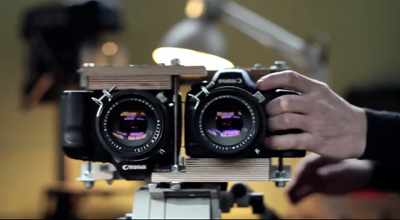
\includegraphics[width=.54\linewidth]{./chapter01/figures/stereo_godard.jpg}} 
\hfill
    \subfloat[La Kinect de @Microsoft qui a permis la d\'emocratisation de 
l'utilisation des capteurs RGB-D]{\label{chap01:fig02view1}
    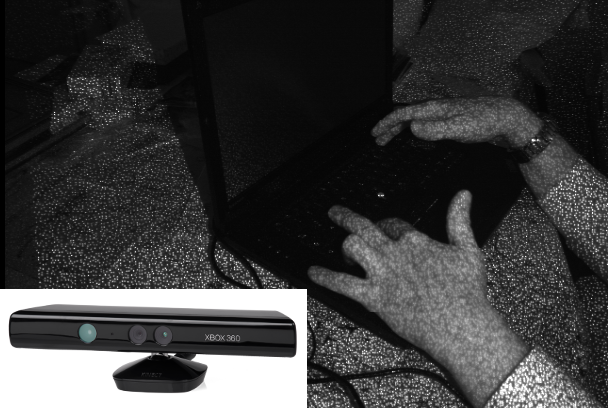
\includegraphics[width=.44\linewidth]{./chapter01/figures/kinect.png}}
    \caption{\footnotesize{Exemples de cam\'eras st\'er\'eo et de capteurs RGB-D.}}
\label{chap01:fig02}
\end{figure}

Une seconde option consiste \`a d\'eterminer les transformations 
g\'eom\'etriques d'ob\-jets dans le plan image g\'en\'er\'ees par une 
modification soit d'une partie de la sc\`ene (objet en mouvement), soit de la 
pose de la cam\'era elle-m\^eme, voire des deux simultan\'ement. Ceci permet 
entre autres de s'abstraire en partie au moins de la repr\'esentation 
tridimensionnelle de la sc\`ene projet\'ee sur l'image, en utilisant par exemple 
la g\'eom\'etrie pl\"uckerienne \cite{andreff:inria-00072393}, des descripteurs 
locaux ou globaux \cite{latuan2010}, ou encore des repr\'esentations 
fr\'equentielles (Fourier \cite{chari2008}, ondelettes \cite{ramosvelasco2012}). 
Le lecteur pourra retrouver les principales techniques dans \cite{marchand2005}.

Le choix d'un type de capteur n'est donc pas anodin, il d\'epend de 
param\`etres aussi divers que la quantit\'e et la densit\'e des informations, 
les connaissances pr\'ealables que l'on peut avoir d'une sc\`ene ou d'un objet, 
du type d'informations disponibles dans l'images et pertinentes par rapport au 
contexte (sc\`enes homog\`enes ou textur\'ees, mobiles ou statiques, diurnes ou 
nocturnes, $\cdots$).

Nous partirons du principe que nous utilisons une seule cam\'era simple, ce 
choix \'etant justifi\'e dans la derni\`ere section de ce chapitre. L'objectif 
est \`a pr\'esent de d\'efinir le mod\`ele de repr\'esentation que nous avons 
utilis\'e, soit la mani\`ere dont la sc\`ene est projet\'ee dans l'image.

\subsection{De la scène à l'image} \label{chap1-0-1}

\subsubsection{Mod\`ele de projection} \label{chap1-0-1-0}

Nous avons privilégié le modèle {\it pinhole} qui offre une approximation 
fiable des caméras perspectives (telles que celles que nous avons utilisées) 
tout en restant formellement simple \cite{Faugeras:1993} \cite{hartley2004}, 
sous les hypothèses du respect des conditions de Gauss (angles de faibles 
incidences), et -- c'est notre cas -- d'une absence de distorsion de la caméra.

Soient ${\bf P} = (X, Y, Z)$ les coordonnées 3-D d'un point dans l'espace et 
${\bf p} = (x_m, y_m)$ ses coordonnées m\'etriques dans l'image. Le modèle de 
projection perspective consiste en une projection centrale de centre $\mathcal 
C$, portée par l'axe ${\bf z}_c$ représentant l'axe optique de la caméra. On 
appelle {\it plan image} le plan se trouvant à distance focale $f$ de la 
caméra, soit $Z = f$. On définit également un point de référence ${\bf c}(x_c,y_c)$ 
dans le plan image comme étant le point d'intersection de l'axe optique et du plan 
image (Fig.\ref{chap01:fig03}).\\

\begin{figure}[h!tp]
  \centering
  \def\svgwidth{.85\linewidth}
  \input{./chapter01/figures/modele_projection.pdf_tex}
    \caption{\footnotesize{Modèle de projection {\it pinhole}}}
\label{chap01:fig03}
\end{figure}

En plus du {\it référentiel-base} $\mathcal R_b$ et du r\'ef\'erentiel de 
l'organe terminal $\mathcal R_e$ (cf. Section \ref{}) s'ajoutent un 
%rajouter reference
{\it référentiel-caméra} noté $\mathcal R_c$, un {\it référentiel-objet} 
$\mathcal R_o$, ainsi qu'un {\it référentiel-image} $\mathcal R_i$. Nous 
noterons également $l_x$ et $l_y$ respectivement la longueur et la hauteur d'un 
pixel dont nous aurons besoin pour la suite.

A partir des coordonnées d'un point ${\bf P}(X, Y, Z)$ exprimées dans le 
référentiel de la caméra, les coordonnées projetées sur le plan images sont 
déduites de la manière suivante :

\begin{equation}
x_m = f \frac{X}{Z}, y_m = f \frac{Y}{Z}
\label{chap01:eq01}
\end{equation}

ou, sous forme matricielle :

\begin{equation}
Z
\begin{bmatrix}
x_m \\y_m \\ 1
\end{bmatrix}
=
\begin{bmatrix}
f & 0 & 0 \\ 0 & f & 0 \\ 0 & 0 & 1 
\end{bmatrix}
\begin{bmatrix}
X \\ Y \\ Z 
\end{bmatrix}
\label{chap01:eq02}
\end{equation}
soit $\widetilde {\bf p} = {\bf A}{\bf P}$, avec $\widetilde {\bf p} = Z {\bf 
p}$.

Un point dans l'image est généralement représenté par ses coordonnées 
pi\-xelliques (l'origine du référentiel étant supposée localisée en haut à 
gauche de l'image).

La conversion entre les coordonnées métriques $(x_m, y_m)$ et les coordonnées 
pixelliques $(x_p, y_p)$, se fait selon la relation suivante :

\begin{equation}
\left \lbrace
\begin{matrix}
x_p = x_c + x_m/l_x \\
y_p = y_c + y_m/l_y
\end{matrix} \right .
\label{chap01:eq03}
\end{equation}
ce qui donne sous une forme matricielle :

\begin{equation}
\begin{bmatrix}
x_p \\y_p \\ 1
\end{bmatrix}
=
\begin{bmatrix}
\frac 1 {l_x} & 0 & x_c \\ 0 & \frac 1 {l_y} & y_c \\ 0 & 0 & 1 
\end{bmatrix}
\begin{bmatrix}
x \\ y \\ 1
\end{bmatrix}
\label{chap01:eq04}
\end{equation}
soit ${\bf p}_p = {\bf B} {\bf p}$.

On obtient la relation suivante entre les coordonnées métriques 3-D du point et 
les coordonnées pixelliques dans l'image :
\begin{equation}
Z\begin{bmatrix}
x_p \\y_p \\ 1
\end{bmatrix}
=
\begin{bmatrix}
\alpha_x & 0 & x_c \\ 0 & \alpha_y & y_c \\ 0 & 0 & 1 
\end{bmatrix}
\begin{bmatrix}
X \\ Y \\ Z
\end{bmatrix}
\label{chap01:eq05}
\end{equation}
avec $\alpha_x = f/l_x$ et $\alpha_y = f/l_y$. Les paramètres $(\alpha_x, 
\alpha_y, x_c, y_c)$ de la matrice ${\bf K} = {\bf A}{\bf B}$ ainsi construite 
sont généralement obtenus par calibration \cite{brown71}, \cite{tsai1986}, 
\cite{stein1997}. La matrice ${\bf K}$ nous permet de faire le lien entre les 
informations géométriques disponibles dans l'image et la projection de la scène 
observée. En particulier, nous pouvons à présent définir les 
coordonnées normalisées ainsi :
\begin{equation}
\left \lbrace
\begin{matrix}
x = X/Z \\
y = Y/Z
\end{matrix} \right .
\label{chap01:eq06}
\end{equation}
indépendantes de la focale, et pouvant être déduites des coordonnées 
pixelliques en utilisant la matrice $\bf K$.

Enfin, les coordonn\'ees 3D du point \'etant exprim\'ees dans le rep\`ere 
cam\'era, nous voulons pouvoir les traduire dans le r\'ef\'erentiel propre de 
l'objet.

\subsubsection{Changements de rep\`ere} \label{chap1-0-1-1}

Soient \`a pr\'esent ${}^c{\bf P} = ({}^cX, {}^cY, {}^cZ)$ les coordonnées du 
point ${\bf P}$ exprimées dans le référentiel $\mathcal R_c$ et ${}^o{\bf P} = 
({}^oX, {}^oY, {}^oZ)$ ses coordonnées dans le référentiel $\mathcal R_o$. Le 
passage d'un référentiel à l'autre est effectué en utilisant la relation 
${}^c{\bf P} = {}^c{\bf t}_o + {}^c{\bf R}_o {}^o{\bf P}$, avec ${}^c{\bf t}_o$ 
le vecteur $3\times 1$ de translation entre les deux référentiels, ${}^c{\bf 
R}_o$ la matrice $3\times 3$ de rotation correspondant à la rotation autour des 
axes du référentiel. En utilisant les coordonnées homogènes $\widetilde {\bf P}$ 
de ${\bf P}$, il est possible de factoriser cette transformation en une seule 
opération matricielle :
\begin{equation}
{}^c \widetilde {\bf P} = {}^c {\bf M}_o {}^o \widetilde {\bf P}
\label{chap01:eq07}
\end{equation}
soit :
\begin{equation}
\begin{bmatrix}
{}^cX \\ {}^cY \\ {}^cZ \\ 1
\end{bmatrix}
=
\begin{bmatrix}
&  {}^c{\bf R}_o & & {}^c{\bf t}_o \\
& {\bf 0} & & 1
\end{bmatrix}
\begin{bmatrix}
{}^oX \\ {}^oY \\ {}^oZ \\ 1
\end{bmatrix}
\label{chap01:eq08}
\end{equation}

On appelle ${}^c{\bf M}_o$ la {\it matrice homogène de transformation} du 
référentiel $\mathcal R_o$ au référentiel $\mathcal R_c$, dont l'inverse 
s'exprime simplement sous la forme :
\begin{equation}
{}^o{\bf M}_c = 
\begin{bmatrix}
&  {}^c{\bf R}_o^T & & -{}^c{\bf R}_o^T {}^c{\bf t}_o \\
& {\bf 0} & & 1
\end{bmatrix}
\label{chap01:eq09}
\end{equation}

En pratique, il suffit de $6$ param\`etres pour d\'ecrire enti\`erement la 
matrice homog\`ene : $3$ pour la translation et $3$ pour la rotation. Si l'on 
utilise par exemple une repr\'esentation des rotations sous la forme ${\bf r} = 
(\theta {\bf u})$, avec $\bf u$ un vecteur unitaire et $\theta$ l'angle de 
rotation autour de ce vecteur, une matrice homog\`ene ${\bf M}$ peut \^etre 
repr\'esent\'ee par le vecteur suivant :

\begin{equation}
{\bf m} = ({\bf t}, \theta {\bf u})  
\label{chap01:eq10}
\end{equation}

Nous sommes \`a pr\'esent en mesure d'établir une relation entre la scène 
observée dans son référentiel propre, dans le r\'ef\'erentiel de la cam\'era (et 
par extension dans chacun des r\'ef\'erentiels du manipulateur) et sa projection 
dans l'image, exprimée en coordonnées pixelliques, métriques et normalisées. Le 
lecteur remarquera cependant que, s'il est possible directement, connaissant 
${\bf K}$ et ${}^o{\bf M}_c$, de déduire à partir des propriétés de la scène 
les caractéristiques de sa projection, l'opération inverse est dépendante dans 
ce modèle d'une estimation pour chaque point de sa profondeur (coordonnée 
${}^cZ$), ce dont nous aurons \`a tenir compte lorsqu'il s'agira de d\'eterminer 
le type de mesures que nous utiliserons pour d\'eduire les consignes \`a donner 
au manipulateur.

\section{Modalit\'es d'asservissement visuel} 
\label{chap1-1}

Selon la nature du manipulateur et le contexte dans lequel celui-ci est 
utilis\'e, plusieurs strat\'egies d'asservissement visuel peuvent \^etre 
utilis\'ees. Nous distinguons en particulier les modalit\'es architecturales 
(positionnement de la cam\'era par rapport au robot et \`a la sc\`ene) et les 
modalit\'es m\'ethodologiques (espace de r\'egulation).

\subsection{Positionnement de la caméra} \label{chap1-1-0}

Lorsque la cam\'era est plac\'ee en dehors de la partie mobile du manipulateur, 
on parlera de configuration déportée (Fig.\ref{chap01:fig04view0}). Une cam\'era 
d\'eport\'ee peut \^etre fixe ou mobile, et permet g\'en\'eralement 
d\'appr\'ehender une sc\`ene d'une mani\`ere globale : elle comporte dans son 
plan image une repr\'esentation de l'organe terminal du robot, et le cas 
\'ech\'eant de l'objet \`a manipuler. L'utilisation d'une cam\'era d\'eport\'ee 
se justifie en particulier lorsque l'on souhaite estimer la pose de l'organe 
terminal par rapport \`a un r\'ef\'erentiel fixe. Toutefois, l'utilisation d'une 
cam\'era d\'eport\'ee -- particuli\`erement si elle est fixe -- suppose une 
sc\`ene relativement d\'egag\'ee et un espace de travail compatible avec son 
champs de vision et sa r\'esolution (il est toujours possible cependant de 
multiplier les dispositifs).

Dans le cas contraire o\`u la cam\'era se trouverait li\'ee \`a l'organe 
terminal d'un manipulateur, on parle en toute logique d'une configuration 
embarquée (Fig.\ref{chap01:fig04view1}). Une cam\'era embarqu\'ee pr\'esente 
l'avantage de pouvoir couvrir l'en\-semble de l'espace de travail accessible au 
manipulateur et de compenser les limites de sa r\'esolution par sa mobilit\'e.

\begin{figure}[htp]
  \centering
  \subfloat[La caméra est déportée ; la scène comprend l'organe terminal et 
l'objet-cible]{\label{chap01:fig04view0}
    \def\svgwidth{.45\linewidth}
  \input{./chapter01/figures/eye_to_hand.pdf_tex}} \hfill
    \subfloat[La caméra est embarquée ; la scène ne comprend que 
l'objet-cible]{\label{chap01:fig04view1}
    \def\svgwidth{.45\linewidth}
  \input{./chapter01/figures/eye_in_hand.pdf_tex}} 
    \caption{\footnotesize{Positionnements de caméra}}
\label{chap01:fig04}
\end{figure}

\subsection{Asservissements en position, basés images et hybrides} 
\label{chap1-1-1}

L'asservissement visuel consiste \`a exploiter les informations visuelles 
situ\'ees dans une image, puis d'en d\'eduire des mesures ${\bf s}$ dont on 
souhaitent qu'elles convergent vers un ensemble de valeurs ${\bf s}^*$ 
correspondant \`a un r\'esultat pr\'edetermin\'e. L'\'ecart entre les valeurs 
mesur\'ees et l'objectif constitue l'erreur ${\bf e}$ de consigne. Cette erreur 
de consigne est alors utilis\'ee pour construire une commande de d\'eplacement 
pour le robot (Fig.\ref{chap01:fig05}). On parle de {\it boucle ouverte} lorsque 
une seule it\'eration est effectu\'ee et suffit \`a produire une consigne 
convergent vers le r\'esultat escompt\'e. On utilise cependant g\'en\'eralement 
un sch\'ema en boucle ferm\'ee consistant \`a mesurer dans chaque nouvelle image 
acquise une correction de la commande. Un sch\'ema en boucle ferm\'e permet de 
prendre en compte les diff\'erentes incertitudes li\'ees \`a la r\'ealit\'e d'un 
d\'eplacement du robot par rapport \`a son mouvement th\'eorique, et permet 
entre autres une robustesse aux erreurs de mesures dans l'image, qui peuvent 
provenir par exemple de la r\'esolution limit\'ee du capteur, ou encore de la 
pr\'esence d'artefacts (ombres, occlusions, $\cdots$).

\begin{figure}[htp]
  \centering
    \def\svgwidth{.95\linewidth}
  \input{./chapter01/figures/bloc_commande.pdf_tex}
    \caption{\footnotesize{Schéma des étapes de l'asservissement visuel}}
\label{chap01:fig05}
\end{figure}

Les informations visuelles \`a partir desquelles sera construite la consigne 
(d\'eplacement exprim\'e dans l'espace op\'erationnel)-- dont on d\'eduira une 
{\it loi de commande} (d\'eplacement exprim\'e dans l'espace articulaire)-- sont 
appel\'ees {\it pri\-mitives}. Selon la nature des primitives, on distingue 
plusieurs types d'asservis\-sement visuels.\\

\noindent {\bf Asservissement 3D :}\\

A partir d'un mod\`ele 3D d'un objet (qui peut-\^etre l'organe terminal) et 
d'une strat\'egie de reconstruction, on cherche \`a estimer la pose courante de 
l'objet par rapport \`a la cam\'era et de la faire converger vers une pose 
d\'esir\'ee, ce que l'on pourra obtenir soit par un mouvement de la cam\'era, 
soit par un d\'eplacement de l'objet. Dans ce cas, ${\bf s}$ correspondra aux 
param\`etres de pose de la cam\'era. On d\'efinit $\mathcal R_c$ et $\mathcal 
R_{c^*}$ comme \'etant respectivement les r\'ef\'erentiels courant et d\'esir\'e 
de la cam\'era, et $\mathcal R_o$ le r\'ef\'erentiel objet. Deux strat\'egies 
peuvent alors \^etre utilis\'ees :
\begin{itemize}
 \item si ${}^c{\bf t}_o$ et ${}^{c^*}{\bf t}_o$ sont les coordonn\'ees de 
l'objet exprim\'ees respectivement dans le r\'ef\'erentiel courant de la 
cam\'era et dans le r\'ef\'erentiel d\'esir\'e, et ${}^{c^o}{\bf R}_c$ la 
matrice de rotation donnant le r\'ef\'erentiel courant par rapport au 
r\'ef\'erentiel d\'esir\'e, alors on a :
 \begin{equation}
 \left \lbrace
 \begin{matrix}
  {\bf s} &=& ({}^c{\bf t}_o,& \theta {\bf u}) \\
  {\bf s}^* &=& ({}^{c^*}{\bf t}_o,& {\bf 0}) \\
  {\bf e} &=& ({}^c{\bf t}_o - {}^{c^*}{\bf t}_o,& \theta {\bf u})
 \end{matrix}
  \right .
\label{chap01:eq11}
\end{equation}
$\theta {\bf u}$ param\'etrisant la matrice de rotation ${}^{c^o}{\bf R}_c$. La 
consigne g\'en\'er\'ee \`a partir de cette repr\'esentation de l'erreur (dont on 
peut trouver le d\'etail dans \cite{chaumette:tuto01}) correspondont \`a une 
trajectoire en ligne droite dans l'image, mais pas pour la cam\'era.
\item au contraire, si on utilise :
\begin{equation}
 \left \lbrace
 \begin{matrix}
  {\bf s} &=& ({}^{c^*}{\bf t}_c,& \theta {\bf u}) \\
  {\bf s}^* &=& (0,& {\bf 0}) \\
  {\bf e} &=& ({}^c{\bf t}_c,& \theta {\bf u})
 \end{matrix}
  \right .
\label{chap01:eq12}
\end{equation}
${}^{c^*}{\bf t}_c$ correspondant ici aux coordonn\'ees du rep\`ere cam\'era 
courant par rapport au rep\`ere cam\'era d\'esir\'e, alors nous obtenons en 
th\'eorie une trajectoire en ligne droite pour la cam\'era, mais pas dans 
l'image. 
\end{itemize}

Ainsi, dans le premier cas, on prend le risque de g\'en\'erer une trajectoire 
pour la cam\'era qui sorte des limites de l'espace de travail, et dans le 
deuxi\`eme cas de voir sortir l'objet de l'image. L'utilisation de l'une ou de 
l'autre m\'ethode impose donc des v\'erifications suppl\'ementaires afin de 
garantir la r\'ealisation de la t\^ache. Aucune des deux solutions ne 
pr\'esentant un clair avantage sur l'autre, le choix d\'ependra du contexte et 
des strat\'egies algorithmiques mises en place.\\

\noindent {\bf Asservissement 2D :} \\

Au contraire de l'asservissement 3D, l'asservissement 2D que l'on retrouve 
\'egalement sous l'acronyme {\it IBVS} (pour {\it Image-based visual servoing}, 
l'asser\-vissement 3D relevant du {\it Position-based visual servoing}) 
exploite directement les primitives extraites des informations visuelles sans 
passer ni par un mod\`ele de la sc\`ene ou de l'objet, ni par une 
reconstruction quelconque. Lorsque la cam\'era se d\'eplace, cela implique 
variations des propri\'et\'es mesurables dans l'image. Si l'on est en capacit\'e 
d\'etablir une relation entre les variations des propri\'et\'es dans l'image et 
les mouvements du capteur, alors il est possible d'obtenir un contr\^oleur qui 
ne repose que sur la r\'egulation des valeurs des primitives. A titre d'exemple, 
sur lequel nous reviendrons dans le prochain chapitre, la mesure de l'aire d'une 
surface et la d\'etermination de son centre de gravit\'e suffisent \`a 
contr\^oler la position d'un manipulateur.

Si un asservissement 2D pr\'esente le clair avantage de proposer une consigne 
d\'etermin\'ee uniquement \`a partir de l'espace du capteur, la construction 
m\^eme de la consigne d\'epend souvent d'estimations suppl\'ementaires telles 
que la profondeur en chaque point. La qualit\'e de l'estimation affectera d\`es 
lors celle de la consigne. Une solution sera par exemple de recourir \`a 
des capteurs suppl\'ementaires pour obtenir ces estimations. 

De mani\`ere g\'en\'erale, le choix d'une primitive visuelle pourra \^etre 
d\'etermin\'e \` partir de quatre crit\`eres :
\begin{itemize}
 \item sa disponibilit\'e dans l'image, sa facilit\'e d'extraction et sa 
robustesse aux variations de l'environnement (luminosit\'e, occlusion, $\cdots$)
  \item son d\'ecouplage par rapport aux degr\'es de libert\'e contr\^ol\'es : 
on souhaite en effet qu'une primitive puisse avoir une r\'eponse forte \`a la 
variation d'un des degr\'es de libert\'e, mais faible aux variations des autres.
  \item son ind\'ependance aux estimations suppl\'ementaires telles que la 
profondeur ou l'orientation du plan de l'image
  \item la convergence du sch\'ema de contr\^ole qui en sera d\'eduit.
\end{itemize}

Le choix d'un ensemble de primitives visuelles prendra donc en compte la 
mani\`ere dont celles-ci se compl\`etent, dans un \'equilibre entre 
d\'ecouplage (pour la robustesse aux erreurs de commande) et redondance (pour 
la compensation des erreurs entre primitives) qui d\'ependra du contexte des 
prises de vue (environnement contr\^ol\'e, dynamique, bruit\'e, $\cdots$).\\

\noindent {\bf Asservissement 2D 1/2 :}\\

Propos\'e par \cite{malis1999}, l'asservissement 2D 1/2 (\'egalement appel\'e 
hybride) combine une approche 2D pour les param\`etres de translation et 3D 
pour les rotations. Pour cela, on utilisera par exemple des points 
d'int\'er\^ets dans l'image, \`a partir desquels on pourra estimer une 
homographie entre l'image courante et une image de r\'ef\'erence. De cette 
homographie seront d\'eduites des mesures permettant de construire ${\bf s}$ \` 
a partir d'informations 2D et 3D, puis de d\'eterminer une consigne -- que 
l'on qualifiera d'hybride -- pour la cam\'era, et enfin une commande pour le 
robot. L'utilisation de l'asservissement 2D 1/2 pr\'esente en particulier 
l'avantage d'offrir un d\'ecouplage des contr\^oles en rotation et en 
translation, mais \'egalement de se dispenser d'une estimation de la profondeur, 
qui sera plut\^ot d\'eduite des homographies successives.


\subsection{Justification des choix de configuration dans le cadre de notre 
\'etude} \label{chap1-1-2}

Nous avons donc le choix des types de capteurs \`a utiliser (cam\'eras 
monoculaires, cam\'eras st\'er\'eos, capteurs RGB-D, $\cdots$), de leur 
disposition, de leur nombre ainsi que de la m\'ethodologie d\'exploitation des 
donn\'ees de l'image et des connaissances {\it a priori} d'une sc\`ene. \\

\noindent {\bf Type de capteurs :}\\

La possibilit\'e d'une reconstruction fid\`ele de la sc\`ene n'en implique 
aucunement la n\'ecessit\'e. En particulier, le robot {\tt Marionet-Assist} sur 
lequel nous avons conduits nos exp\'erimentations a \'et\'e con\c cu dans un 
cadre de robotique de service et d'assistance, d\'eployable donc dans des 
environnements priv\'es (domicile de l'utilisateur ou chambre d'h\^opital par 
exemple). A ce titre, se pose la question de l'intimit\'e et du respect de la 
vie priv\'ee des utilisateurs. Si nous pouvons r\'ealiser avec une cam\'era 
monoculaire les mesures n\'ecessaires \`a la r\'ealisation d'une t\^ache sans 
efforts suppl\'ementaires d\'emesur\'es, ce choix doit \^etre privil\'egi\'e. 
La question n'est pas tant ici de faire mieux avec plus, mais de faire autant 
avec moins, en utilisant les propri\'et\'es des robots \`a c\^ables pour 
obtenir des lois de commande simplifi\'ees et n\'eanmoins pr\'ecises et 
robustes.\\

\noindent {\bf Disposition et nombre des capteurs :}\\

Les robots parall\`eles \`a c\^ables se distinguent par la taille de leur 
espace de travail g\'en\'eralement cons\'equente. A titre d'exemple, le robot 
{\tt Marionet-As\-sist} évolue dans un cube de $4m \times 3m \times 3m$, et le 
volume atteignable par un robot de type {\tt Marionet-Crane} peut aller jusqu'à 
$100m \times 35m \times 35m$. D\`es lors, l'utilisation d'une seule cam\'era 
d\'eport\'ee sera probablement insuffisante pour couvrir l'ensemble de l'espace 
atteignable par le manipulateur. Les solutions envisageables sont donc 
l'utilisation de plusieurs dispositifs d\'eport\'es, d'un dispositif 
embarqu\'e, ou d'un dispositif embarqu\'e compl\'et\'e par un ou plusieurs 
dispositifs d\'eport\'es. Puisque les robots {\tt Marionet} ont \'egalement 
vocation \`a \^etre utilis\'es dans des environnements dynamiques et/ou inconnus 
(pi\`eces de vie, catastrophe naturelle, $\cdots$), il nous semble opportun 
d'assurer la pr\'esence d'au moins un capteur embarqu\'e, afin de pouvoir 
contourner d'eventuels obstacles, ou de pouvoir s'approcher suffisamment pr\`es 
d'une sc\`ene pour compenser d'\'eventuelles limites de r\'esolution. La 
question se pose alors de savoir si une seule cam\'era embarqu\'ee suffit, ou 
s'il est n\'ecessaire de compl\'eter le dispositif avec d'autres capteurs 
d\'eport\'es.

Pour assurer la saisie et la manipulation d'un objet, nous montrerons au 
chapitre suivant qu'une cam\'era embarqu\'ee suffit \`a la convergence de la 
t\^ache d'asservissement. Toutefois, nous avons vu que la jacobienne du robot, 
qui peut \^etre utilis\'ee soit pour un contr\^ole cin\'ematique, soit pour 
v\'erifier l'\'equilibre statique, \'etait d\'ependante de la pose et des 
coordonn\'ees articulaires. Une cam\'era d\'eport\'ee peut donc s'av\'erer 
judicieuse pour servir de capteur ext\'eroceptif. Nous verrons dans la 
derni\`ere section de ce chapitre que cette piste a \'et\'e \'etudi\'ee et 
fournit des r\'esultats tout-\`a-fait int\'eressants.

Toutefois, nous montrerons que notre sch\'ema d'asservissement est robuste aux 
erreurs de mod\'elisations, et donc qu'une estimation pr\'ecise de la pose ou 
des longueurs de c\^ables n'est pas n\'ecessaire. Dans une version simplifi\'ee 
de la commande utilis\'ee pour l'asservissement, nous verrons d'ailleurs que 
nous pouvons nous passer en partie des param\`etres de pose et des 
coordonn\'ees articulaires.

Nous prenons donc le parti dans ce travail de ne travailler qu'avec une seule 
cam\'era embarqu\'ee.\\

\noindent {\bf Strat\'egie d'asservissement :}\\

Une cam\'era embarqu\'ee suffit pour pouvoir utiliser une strat\'egie PBVS en 
multipliant les points de vue, et est totalement adapt\'ee aux asservissements 
2D et hybrides. Pour autant, lorsque nous \'evoquerons les travaux existants 
sur l'asservissement des robots parall\`eles \`a c\^ables, nous verrons que 
l'asservissement 3D a d\'ej`a \'et\'e explor\'e et a donn\'e des r\'esultats 
tout-\`a-fait convaincants. D\`es lors, nous nous concentrerons ici sur les 
asservissements 2D afin de compl\'eter l'\'etat de l'art, l'extension aux 
asservissements hybrides ne pr\'esentant pas de difficult\'e suppl\'ementaire. 
En particulier, un choix particulier de primitives -- les moments 2D -- nous 
permettra de ne pas nous appuyer sur des mesures suppl\'ementaires, telles 
l'estimation de la profondeur.

\section{D\'etermination du sch\'ema de consigne}\label{chap1-2}

Nous reprenons ici les bases de construction d'une loi de commande 
\cite{samson1991}. Le lecteur les retrouvera développées par exemple dans 
\cite{chaumette2008handbook}. Nous nous contentons ici d'exposer les principes 
généraux d'outils que nous avons utilisés tout au long de nos travaux.

\subsection{Construction de la loi de commande}

Soient ${\bf s}(m(t), a)$ un vecteur comprenant de mesures $m(t)$ réalisées au 
sein de l'image sur des primitives choisies et $a$ la param\'etrisation de 
connaissances {\it a priori}, telles les param\`etres intrins\`eques de la 
cam\'era ou encore des connaissances pr\'ealable sur la sc\`ene ou l'objet 
cibl\'e. Le vecteur ${\bf s}^*$ d\'enote les valeurs désirées des mesures.

On construit alors le vecteur :
\begin{equation}
{\bf e} = {\bf s} - {\bf s}^*
\label{chap01:eq13}
\end{equation}
représentant une erreur correspondant \`a la différence entre les valeurs 
courantes et les valeurs désirées.

Nous souhaitons que l'erreur ${\bf e}$ de mesure décroisse de manière 
exponentielle, soit :
\begin{equation}
\dot {\bf e} = - \lambda {\bf e}
\label{chap01:eq14}
\end{equation}
$\lambda$ étant un {\it gain}, permettant de régler la vitesse de convergence.

On choisit ici d'utiliser un contr\^ole en vitesse. Soit le torseur cinématique 
$\bv_c = (\bnu_c, \bomega_c)$, avec $\bnu_c$ et $\bomega_c$ les vitesses 
instantanées respectivement linéaires et angulaires exprim\'ees dans le 
r\'ef\'erentiel-cam'era. Il est nécessaire dans un premier temps de déterminer 
les variations $\dot {\bf s}$ des mesures pour un déplacement donné $\bv_c$ de 
la caméra. Cette relation peut prendre la forme algébrique d'une matrice ${\bf 
L}_s \in \mathcal M_{k\times 6}$ que l'on appelle {\it matrice d'interaction} 
\cite{espiau1992}, $k$ \'etant le nombres de mesures effectuées. Nous avons 
alors la relation :
\begin{equation}
\dot {\bf s} = {\bf L}_s \bv_c
\label{chap01:eq15}
\end{equation}

En combinant (Eq.\ref{chap01:eq13}) et (Eq.\ref{chap01:eq15}), la relation 
entre la variation de l'erreur et la vitesse de la cam\'era se d\'eduit 
imm\'ediatement :
\begin{equation}
\dot {\bf e} = {\bf L}_e \bv_c
\label{chap01:eq16}
\end{equation}
avec ${\bf L}_e = {\bf L}_s$.

D\`es lors, (Eq.\ref{chap01:eq14}) et (Eq.\ref{chap01:eq16}) nous 
donnent :
\begin{equation}
{\bv}_c = - \lambda {\bf L}^+_e {\bf e}
\label{chap01:eq17}
\end{equation}
avec ${\bf L}^+_e$ pouvant \^etre de plusieurs natures :
\begin{itemize}
 \item lorsque $k \geq 6$ et que la matrice ${\bf L}_e$ est de rang plein, 
${\bf L}^+_e$ correspondra \`a la matrice pseudo-inverse de Moore-Penrose de 
${\bf L}_e$, soit ${\bf L}^+_e = ({\bf L}_e^T{\bf L}_e)^{-1}{\bf L}_e^T$.
\item lorsque $k = 6$ et que le d\'eterminant de la matrice d'interaction est 
non-nul, on pourra \'ecrire $\dot {\bv}_c = - \lambda {\bf L}^{-1}_e {\bf e}$.
\end{itemize}


\subsection{Exemple de construction d'une matrice d'interaction : le point}

Pour rappel, un point dans l'espace ${\bf P} = (X, Y, Z)$ se projette dans 
l'image de la mani\`ere suivante :

\begin{equation}
\left \lbrace
\begin{matrix}
x = X/Z \\
y = Y/Z 
\end{matrix}
\right .
\label{chap01:eq17}
\end{equation}
o\`u $(x,y)$ sont les coordonn\'ees g\'en\'eralis\'ees du point dans l'image.

En d\'erivant cette relation, nous obtenons :
\begin{equation}
\left \lbrace
\begin{matrix}
\dot x = \dot X/Z - X \dot Z/Z^2  = (\dot X - x \dot Z)/Z \\
\dot y = \dot Y/Z - Y \dot Z/Z^2  = (\dot Y - y \dot Z)/Z 
\end{matrix}
\right .
\label{chap01:eq18}
\end{equation}

Soit $\bv = (\bnu, \bomega)$ le torseur cin\'ematique de la cam\'era, la 
relation permettant d'exprimer la vitesse du point ${\bf X}$ par rapport \`a la 
vitesse de la cam\'era s'\'ecrit :

\begin{equation}
\dot {\bf X} = -\bv - \bomega \times {\bf X}
\label{chap01:eq19}
\end{equation}
soit :
\begin{equation}
\left \lbrace
\begin{matrix}
\dot X = -\bnu_x - \bomega_y Z + \bomega_z Y \\
\dot Y = -\bnu_y - \bomega_z X + \bomega_x Z \\
\dot X = -\bnu_z - \bomega_x Y + \bomega_y X \\
\end{matrix}
\right .
\label{chap01:eq20}
\end{equation}

D\`es lors, en combinant (Eq.\ref{chap01:eq18}) et (Eq.\ref{chap01:eq20}), on 
obtient :
\begin{equation}
\left \lbrace
\begin{matrix}
\dot x &=& -\bnu_x/Z +x\bnu_z/Z + xy\bomega_x -(1+x^2)\bomega_y + y \bomega_z \\
\dot y &=& -\bnu_y/Z +y\bnu_z/Z + (1+y^2)\bomega_x -xy\bomega_y - x \bomega_z
\end{matrix}
\right .
\label{chap01:eq21}
\end{equation}

La matrice d'interaction ${\bf L}_x$ reliant la vitesse du point ${\bf x} = 
(x,y)$ au torseur cin\'ematique de la cam\'era est alors :

\begin{equation}
{\bf L}_x =
\begin{bmatrix}
\frac {-1} Z & 0 & \frac x Z & xy & -(1+x^2) & y \\
0 & \frac {-1} Z & \frac y Z & 1+y^2 & -xy & -x
\end{bmatrix}
\label{chap01:eq22}
\end{equation}
soit bien $\dot {\bf x} = {\bf L}_x \bv$.

Afin de contr\^oler $6$ degr\'es de libert\'e, $3$ points au minimum sont 
n\'ecessaires, mais la matrice pourra alors en certaines poses se r\'ev\'eler 
singuli\`ere \cite{michel1993}. il existe de plus plusieurs minima locaux 
conduisant \`a ${\bf e} = 0$. Pour ces deux raisons, on utilisera $4$ points au 
moins pour contr\^oler le manipulateur.\\

De plus, la matrice \'etant exprim\'ee dans les coordonn\'ees 
g\'en\'eralis\'ees, elle d\'epend des param\`etres de la cam\'era. Elle 
n\'ecessite enfin une approximation de $Z$, et ceci pour chaque point 
permettant de construire la matrice d'interaction. En cons\'equence, la matrice 
th\'eorique que nous venons d'expliciter ne peut \^etre utilis\'ee en l'\'etat, 
nous recourrons donc \`a une approximation.

\subsection{Choix d'approximation de la matrice d'interaction et crit\`ere de
convergence}

Devant la difficult\'e en pratique de connaître avec exactitude ${\bf 
L}_e$, on utilisera plut\^ot une approximation de la matrice d'interaction, la 
loi de commande finale devenant :
\begin{equation}
{\bf v}_c = - \lambda \widehat {{\bf L}_e^+} {\bf e} 
\label{chap01:eq23}
\end{equation}











\section{Asservissement visuel des robots parallèles à 
câbles}\label{chap1-3}

Nous avons vu que plusieurs caract\'eristiques des robots parall\`elles
\`a c\^ables peuvent alt\'erer la qualit\'e de la manipulation. Ainsi, la
complexit\'e des mod\`eles g\'eom\'etriques et cin\'ematiques par rapport aux
robots s\'eries et aux robots parall\`eles rigides menace d'une part la
pr\'ecision des op\'erations de manipulation lors de la r\'esolution
num\'erique, et d'autre part l'effectuation en temps r\'eel. De plus, la
n\'ecessaire v\'erification de l\'equilibre statique pour toutes les
configurations de c\^ables en tension strictement positive impacte \'egalement
la contrainte de r\'ealisation en temps r\'eel d'une t\^ache ; surtout, il est
tout autant difficile de pr\'evoir quels c\^ables seront en tension lors d'un
d\'eplacement prescrit, que de garantir la constance du caract\`ere positif ou
nul de la tension d'un c\^able sur l'int\'egralit\'e d'un d\'eplacement. Enfin,
les incertitudes m\'ecaniques -- telles par exemple le diam\`etre r\'eel de la
couche d'enroulement d'un c\^able autour des tambours -- ont \'egalement une
influence sur la pr\'ecision du manipulateur.

Il est donc n\'ecessaire, afin de garantir l'efficacit\'e d\'une t\^ache de
manipulation, de simplifier la r\'esolution num\'erique des mod\`eles, de
d\'evelopper une strat\'egie de contr\^ole de la tension dans les diff\'erents
c\^ables, et de corriger enfin la trajectoire du manipulateur lorsque les
incertitudes et erreurs perturbent celle-ci.

L'utilisation de capteurs suppl\'ementaires a \'et\'e propos\'ee \`a de
nombreuses reprises afin de r\'esoudre un ou plusieurs des probl\`emes
\'enonc\'es. Dans le contexte des robots parall\`eles \`a jambes rigides,
plusieurs suggestions ont \'et\'e faites :
\begin{itemize}
 \item mesurer directement la pose de l'organe terminal \`a l'aide de
syst\'emes de lasers et miroirs \cite{marantette1995machine}, \cite{Heeren:1992}
ou d'une cam\'era d\'eport\'ee \cite{dallej.2006}, \cite{paccot.2008} : cela
permet tout autant une simplification des mod\`eles qu'une correction des
erreurs et impr\'ecisions.
\item utiliser des capteurs proprioceptifs afin d'obtenir une repr\'esentation
fid\`ele de l'\'etat des variables articulaires
\cite{merlet.1993}, \cite{parenti.2000}, ce qui permet \'egalement une
simplification des mod\`eles pouvant aboutir \`a une ex\'ecution en temps
r\'eel. 
\item un contr\^ole r\'ef\'erenc\'e vision bas\'e sur l'exploitation de mesures
des directions des jambes du robot \cite{andreff2007} : dans cette derni\`ere
m\'ethode, une strat\'egie IBVS est utilis\'ee pour d\'efinir un contr\^ole
cin\'ematique. Elle permet de s'affranchir du calcul du MGD, ce qui la rend
{\it a priori} robuste aux erreurs de mod\`eles et de calibrations.
\end{itemize}

En particulier, cette derni\`ere m\'ethode a \'et\'e d\'eclin\'ee r\'ecemment
pour le contr\^ole de robots parall\`eles \`a c\^ables. Elle fait suite \`a
une premi\`ere approche \cite{conf/iros/DallejGAMM11} consistant \`a mettre dans
un premier temps en place un asservissement visuel 3-D (PBVS) sur l'organe
terminal, puis \`a \'elaborer un sch\'ema de contr\^ole dynamique utilisant la
vision pour estimer la pose et la v\'elocit\'e de la plate-forme. Malgr\'e des
r\'esultats prometteurs obtenus en simulation, il reste \`a valider cette
approche sur un prototype r\'eel.

Les m\^emes auteurs ont donc par la suite propos\'e une approche analogue au
suivi de jambes des robots parall\`eles classiques \cite{dallej2012}, en
exploitant cette fois-ci les directions de d\'eparts des c\^ables, compl\'etant
ainsi un syst\`eme de mesures utilisant des capteurs de forces (afin d'estimer
la tension dans les c\^ables), ainsi que plusieurs cam\'eras d\'eport\'ees pour
estimer la pose de la plate-forme. Le sch\'ema d'ensemble utilise donc un 
premier
ensemble de quatre cam\'eras filmant un motif sur l'organe terminal pour
proposer un asservissement 3-D donnant le torseur cinem\'atique de l'organe
terminal, puis quatre cam\'eras st\'er\'eos donnant la direction tangente aux
d\'eparts de c\^ables, permettant ainsi de simplifier le contr\^ole
cin\'ematique du robot. A nouveau, les r\'esultats pr\'esent\'es en simulation
nous paraissent tout-\`a-fait prometteurs, mais doivent encore \`a notre
connaissance \^etre valid\'es exp\'erimentalement.

Nous avons toutefois choisi de ne pas poursuivre dans la m\^eme voie pour
les trois raisons suivantes :
\begin{itemize}
 \item pour des raisons d'intrusivit\'e et de co\^ut propres aux conditions
d'applications des prototypes sur lesquels nous avons travaill\'e, le
dispositif de mesure nous a paru trop cons\'equent ; nous avons
de plus privil\'egi\'e des configurations embarqu\'ees comme mentionn\'e
pr\'ec\'edemment.
\item bien qu'ils fassent durant leurs travaux l'hypoth\`ese de c\^ables
non-\'elastiques, les auteurs supposent une pr\'ecision des mesures de tension
qui nous semble difficilement atteignable pour des robots de cette envergure. Il
ne s'agissait \'evidemment pas du sujet de leur \'etude, mais nous pensons
n\'eanmoins que certaines situations que nous avons rencontr\'ees pourraient
affecter la qualit\'e des r\'esultats annonc\'es. 
\item enfin, le sch\'ema de contr\^ole repose sur l'estimation et l'inversion
de la matrice d'interaction d'une part, et sur l'estimation de la Jacobienne
inverse d'autre part, se pr\'esentant donc sous la forme :
\begin{equation}
\dot {\bf q} = - \lambda \widehat {{\bf J}^{-1}} \widehat{ {\bf L}_e^+} {\bf e} 
\label{intro:eq25}
\end{equation}
Nous pensons qu'il est possible d'unifier ces deux \'etapes \`a la condition
d'ex\'ecuter un contr\^ole cin\'ematique \`a l'aide d'une cam\'era embarqu\'ee,
soit une seule matrice :
\begin{equation}
\dot {\bf q} = - \lambda \widehat {\bf K} {\bf e} 
\label{intro:eq26}
\end{equation}
ne n\'ecessitant pas plus de connaissance pr\'ecise de la pose $X$ que des
valeurs des variables articulaires $\rho$.
\end{itemize}

Bien que nous ne puissions garantir que cette simplification du sch\'ema de
contr\^ole puisse s'appliquer \`a toutes les configurations de robots \`a
c\^ables, elle s'av\`ere efficace dans notre contexte, particuli\'erement pour
les robots $N-1$. Sa mise en place implique toutefois certaines conditions qui
peuvent se r\'ev\'eler incompatibles avec un ensemble d'applications, ce que
nous exposerons lors du chapitre qui sera consacr\'e \`a son \'etude.

Le travail qui est pr\'esent\'e ici a pour objectif d'am\'eliorer la qualit\'e
de manipulation d'un robot parall\`ele \`a c\^ables. Pour cela, nous avons
distingu\'e quatre crit\`eres qui nous permettront d'\'evaluer notre
contribution, \`a savoir :
\begin{enumerate}
 \item la {\bf stabilit\'e} de la plate-forme lors d'un d\'eplacement
 \item la {\bf pr\'ecision} de la pose finale
 \item la {\bf robustesse} aux impr\'ecisions et erreurs de mod\`ele, aux
erreurs et impr\'ecisions des estimations des param\`etres de contr\^ole
  \item la {\bf simplicit\'e} du sch\'ema de contr\^ole
\end{enumerate}

Dans ce but, nos travaux seront pr\'esent\'es de la mani\`ere suivante : 
\begin{itemize}
 \item dans un premier temps, nous pr\'esenterons une strat\'egie de contr\^ole
des c\^ables en tension, qui nous permettra d'am\'eliorer la stabilit\'e des
mouvements, ainsi que la pr\'ecision des d\'eplacements.
 \item une fois cette stabilit\'e assur\'ee, nous montrerons que l'utilisation
d'un asservissement visuel am\'eliore la pr\'ecision du positionnement de
l'organe terminal, mais \'egalement la robustesse du contr\^ole
 \item nous utiliserons ensuite les sp\'ecificit\'es des architectures
parall\`eles pour d\'evelopper une loi de contr\^ole simplifi\'ee, ce qui nous
permettra de gagner ici en robustesse et en simplicit\'e de calcul.
 \item enfin, un chapitre pr\'esentera plusieurs simulations et
exp\'erimentations sur notre prototype. Ceci nous permettra de valider nos
diff\'erentes approches, mais \'egalement d'en pr\'esenter les limites, ce qui
nous permettra en conclusion de faire le point sur les perspectives s'ouvrant
en continuit\'e de ces travaux.
\end{itemize}




Enfin, il était envisageable dans cette étude d'utiliser les caméras soit comme 
capteur intéroceptif, soit comme capteur extéroceptif. Le choix d'une 
observation des articulations d'un robot parallèle à câbles a été effectué par 
\cite{andreff2007} pour des robots parallèles classiques, et plus récemment 
pour des robots parallèles à câble \cite{dallej2011}, \cite{dallej2012}. Ces 
études 
correspondant à ce jour au principal travail effectué dans le domaine de 
l'asservissement visuel des robots parallèles à câbles, nous reviendrons dès 
lors dessus à l'occasion de la section suivante, au sein de laquelle nous 
définirons nos problématiques et pistes de travail. Nous pouvons relever 
toutefois que la démarche développée dans leurs recherches consiste à améliorer 
le positionnement de l'organe terminal, ce qui suppose que la position de la 
cible est connue avec suffisamment de précision. Il s'agit donc d'un 
environnement contrôlé. Or, le contexte d'application de nos robots implique au 
contraire une incertitude non-négligeable sur les propriétés de la cible. Dès 
lors, la caméra est tout autant utilisée pour la construction d'une loi de 
commande que pour la localisation de l'objet et l'actualisation de ses 
propriétés lorsque celles-ci diffèrent d'une première estimation. Le choix 
d'utilisation des caméras comme capteurs extéroceptifs s'est donc imposé dans 
notre approche.





